% latex2e header
\documentclass[11pt]{article}
\usepackage{latexsym}
\usepackage{fullpage}
\usepackage{fancyhdr}
\usepackage{graphicx}
%\usepackage{pstricks}
%\usepackage{psfig}
%\pagestyle{fancyplain}
\pagestyle{empty}
\topmargin   -0.70in

%\input{lab-fmt.tex}
\input epsf.sty
%\setcounter{laboratory}{2} %one less
\def\half{{\textstyle {1\over2}}}
\def\3half{{\textstyle {3\over2}}}

\setlength{\textheight}{10.5in}


\begin{document}
\thispagestyle{empty}
Professor Fearing ~~~~~~~~~~ EECS 192 Note on DT Control, 4/7/2015 v1.01~~~~~~~~~~~ Spring 2015\\



Consider a first order continuous time linear system with dynamics given by:
\begin{equation}
\dot{x} = -x + u
\end{equation}

In discrete time, a ``zero-order-hold'' holds the 
value of the control input $u(t)$ constant for one time step $T$, i.e.
the control $u(t) = u(kT)$ for $kT \le t < kT+T$.

Let the error $e(t) = r(t) - x(t)$, and a feedback controller
is chosen such that $u(t) = 3(x(t) - r(t))$ where $r(t)$ is the reference.
Here $r(t)$ is the unit step.

Assume the system has initial condition $x(0) = 0$. The state and error are listed
in the table below at each $T$. Note that the system is continuous,
but the control value is held constant and updated at each $T$.\\

\begin{tabular}{cccc}
t (sec) & x(t) & e(t) = r(t) - x(t) & u(t) \\
\hline
\hline
$0^-$ & 0 & 0 & 0 \\
0 & 0 & 1 & 3\\
1 & 2 & -1 & -3\\
2 & -1 & 2 & 6\\
3 & 3.5 & -2.5 & -7.5\\
4 & -3.5 & 4.5 & 13.5\\
5 & 6.5 & -5.5 & -16.5
\end{tabular}

This example is unstable. By reducing the sampling period, 
(even while keeping the gain the same), the control system can be made stable.

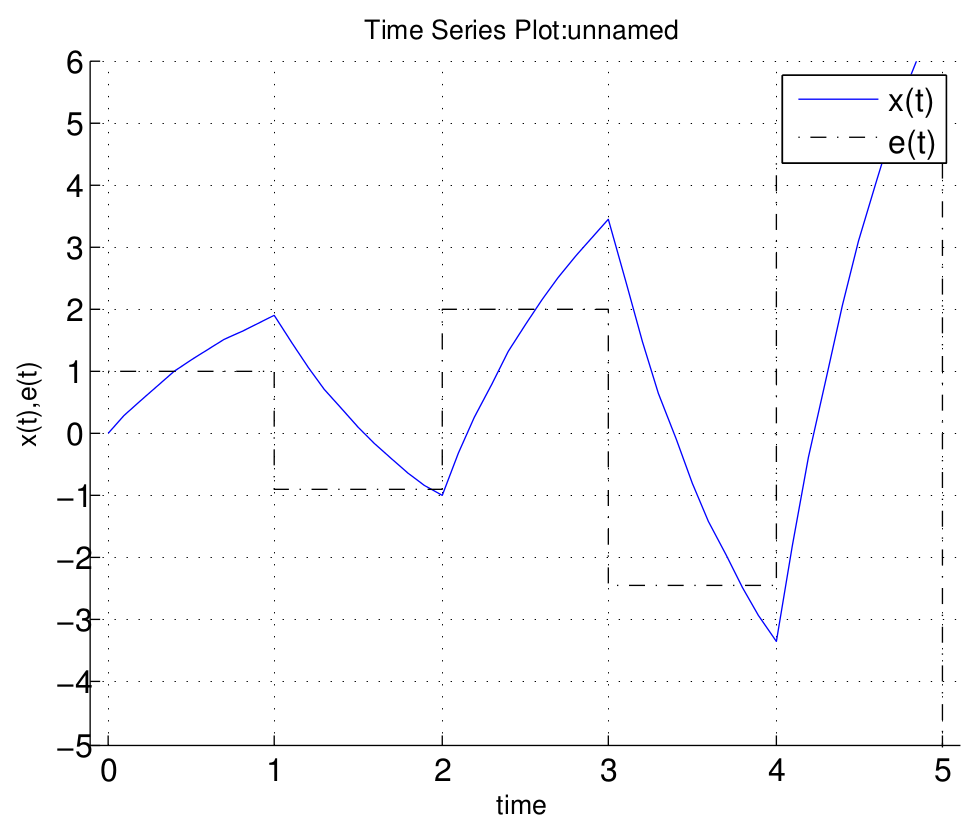
\includegraphics[scale=0.5]{dt-unstable.png}


\end{document}

